%% 
%% Copyright 2019-2024 Elsevier Ltd
%% 
%% This file is part of the 'CAS Bundle'.
%% --------------------------------------
%% 
%% It may be distributed under the conditions of the LaTeX Project Public
%% License, either version 1.3c of this license or (at your option) any
%% later version.  The latest version of this license is in
%%    http://www.latex-project.org/lppl.txt
%% and version 1.3c or later is part of all distributions of LaTeX
%% version 1999/12/01 or later.
%% 
%% The list of all files belonging to the 'CAS Bundle' is
%% given in the file `manifest.txt'.
%% 
%% Template article for cas-sc documentclass for 
%% double column output.

\documentclass[a4paper,fleqn]{cas-sc}

% If the frontmatter runs over more than one page
% use the longmktitle option.

%\documentclass[a4paper,fleqn,longmktitle]{cas-sc}

%\usepackage[numbers]{natbib}
%\usepackage[authoryear]{natbib}
\usepackage[authoryear,longnamesfirst]{natbib}

%%%Author macros
\def\tsc#1{\csdef{#1}{\textsc{\lowercase{#1}}\xspace}}
\tsc{WGM}
\tsc{QE}
%%%

% Uncomment and use as if needed
%\newtheorem{theorem}{Theorem}
%\newtheorem{lemma}[theorem]{Lemma}
%\newdefinition{rmk}{Remark}
%\newproof{pf}{Proof}
%\newproof{pot}{Proof of Theorem \ref{thm}}

\begin{document}
\let\WriteBookmarks\relax
\def\floatpagepagefraction{1}
\def\textpagefraction{.001}

% Short title
\shorttitle{}    

% Short author
\shortauthors{}  

% Main title of the paper
\title [mode = title]{}  

% Title footnote mark
% eg: \tnotemark[1]
% \tnotemark[1] 

% Title footnote 1.
% eg: \tnotetext[1]{Title footnote text}
% \tnotetext[1]{} 

% First author
%
% Options: Use if required
% eg: \author[1,3]{Author Name}[type=editor,
%       style=chinese,
%       auid=000,
%       bioid=1,
%       prefix=Sir,
%       orcid=0000-0000-0000-0000,
%       facebook=<facebook id>,
%       twitter=<twitter id>,
%       linkedin=<linkedin id>,
%       gplus=<gplus id>]

% \author[1]{}%[<options>]

% Corresponding author indication
% \cormark[1]

% Footnote of the first author
% \fnmark[1]

% Email id of the first author
% \ead{}

% URL of the first author
% \ead[url]{}

% Credit authorship
% eg: \credit{Conceptualization of this study, Methodology, Software}
% \credit{}

% Address/affiliation
% \affiliation[1]{organization={},
%             addressline={}, 
%             city={},
%          citysep={}, % Uncomment if no comma needed between city and postcode
            % postcode={}, 
            % state={},
            % country={}}

% \author[2]{}%[]

% Footnote of the second author
% \fnmark[2]

% Email id of the second author
% \ead{}

% URL of the second author
% \ead[url]{}

% Credit authorship
% \credit{}

% Address/affiliation
% \affiliation[2]{organization={},
%             addressline={}, 
%             city={},
%          citysep={}, % Uncomment if no comma needed between city and postcode
            % postcode={}, 
            % state={},
            % country={}}

% Corresponding author text
% \cortext[1]{Corresponding author}

% Footnote text
% \fntext[1]{}

% For a title note without a number/mark
%\nonumnote{}

% Here goes the abstract
\begin{abstract}
Here goes the abstract.
\end{abstract}

% Use if graphical abstract is present
%\begin{graphicalabstract}
%\includegraphics{}
%\end{graphicalabstract}

% Research highlights
% \begin{highlights}
% \item 
% \item 
% \item 
% \end{highlights}


% Keywords
% Each keyword is seperated by \sep
\begin{keywords}
 \sep \sep \sep
\end{keywords}

\maketitle

% Main text
\section{Introduction}\label{sec:introduction}

This study investigates how the effects of AI NPC personality extend from individual interaction to dyadic collaboration, and how NPC personality and pair familiarity jointly influence users’ perceptions of the AI, reliance on the AI, and collaborative engagement in dyadic settings.

%% The Appendices part is started with the command \appendix;
%% appendix sections are then done as normal sections
%% \appendix

\section{Related Work}\label{sec:related-work}

\subsection{AIMR in museum contexts}
Museums serve both entertainment and educational functions. 
Due to the specialty of MR, museum can provide a more immersive experience and shorten the distance between visitors and artifacts. On the other hand, AI can 

XXX shows that Guide can , while XXX shows that AI . Highlighting that AI.

\subsection{personality traits via LLM}
There is research showing that CAs with personality design can enhance social presence \citep{Ahmadetal2021}.

Under this research trend, the Big Five Personality Model proposed by Oliver P. \cite{John1991} is the most widely adopted framework in contemporary psychology. There are five traits, and extraverison. Each represents and used to evaluate.

Among the five personality traits, Extraversion has been evaluated as the most affected personality dimension for several reasons \citep{GillOberlander2019}.

\subsection{team structure (acquainted vs. unacquainted pairs) in HAI}

\section{Lab Experiment: Single User}\label{sec:lab}

This study uses a within-subjects MR tour experiment to examine the effects of introverted and extroverted NPCs on multiple dependent variables, enabling a comparative evaluation while minimizing individual differences.

\subsection{Method}

Participants first completed the BFI-2 personality test and were classified as introverts (scores $\leq 36$) or extroverts (scores $>36$). Sixteen participants, with eight participants in each group and ages ranging from 20 to 30 years, were recruited for the study. Manipulation checks conducted during the pilot test confirmed that the two AI NPCs exhibited significantly different perceived personalities. The extroverted AI NPC was described as `enthusiastic` and `energetic`, whereas the introverted AI NPC was described as `calm` and `disciplined`.

After receiving a study briefing and reviewing example questions, participants were randomly assigned to one of two interaction orders. Each participant wore a HoloLens mixed-reality headset and interacted with both AI NPCs for up to eight minutes per NPC. Each interaction session began with a self-introduction by the NPC, followed by two predefined questions.

After interacting with both NPCs, participants completed a knowledge task designed to ensure sufficient engagement with the study content. Participants who scored below 80\% were excluded from the analysis. The study concluded with a post-experiment questionnaire and a short interview. The complete procedure lasted approximately 35--40 minutes.

\subsection{Questionnaire}
Before interacting with the AIMR system, participants' levels of extraversion were assessed using the BFI-2 pre-test questionnaire. The resulting extraversion scores served as a key variable for testing the similarity-attraction effect proposed in Hypothesis~4. To capture participants' perceptions and experiences, subjective data were collected through post-experiment questionnaires using a five-point Likert scale. The questionnaire measured social presence (SP), purchase intention (PI), continuance intention to use (ITU), and satisfaction (SAT).

Social presence was measured using five items adapted from Gefen and Straub~\cite{GefenStraub2004}, which demonstrated satisfactory reliability and convergent validity ($\mathrm{CR}=0.919$, $\sqrt{\mathrm{AVE}}=0.836$). These subjective evaluations were complemented by objective measures, including eye-tracking data and interaction frequency. Purchase intention was measured using items adapted from Barta et al.~\cite{Bartaetal2023} (Cronbach's $\alpha=0.958$, $\rho_{c}=0.973$, $\mathrm{AVE}=0.922$). Continuance intention to use was measured using items adapted from Li and Wang~\cite{LiWang2023} (Cronbach's $\alpha=0.93$, $\mathrm{AVE}=0.78$, $\mathrm{CR}=0.94$). Satisfaction was assessed using items adapted from Shi et al.~\cite{Shietal2023} ($\mathrm{CR}=0.910$, $\mathrm{AVE}=0.717$). These reported values indicate strong reliability and convergent validity across the measured constructs.

The questionnaire also included open-ended questions to enrich the qualitative findings and capture participants' perceptions of social presence, continuance intention to use, purchase intention, and visual attention. For social presence, participants identified which NPC conveyed a stronger sense of ``being there'' and explained the reasons for their choice. For continuance intention to use, they described why they would prefer to interact with a particular AI NPC in the future. For purchase intention, they indicated whether the interaction increased their motivation to purchase museum souvenirs and explained why. Regarding visual attention, participants described moments in which an AI NPC's remarks prompted them to examine an exhibit more closely.

\subsection{Behavioral}
\begin{figure}
    \centering
    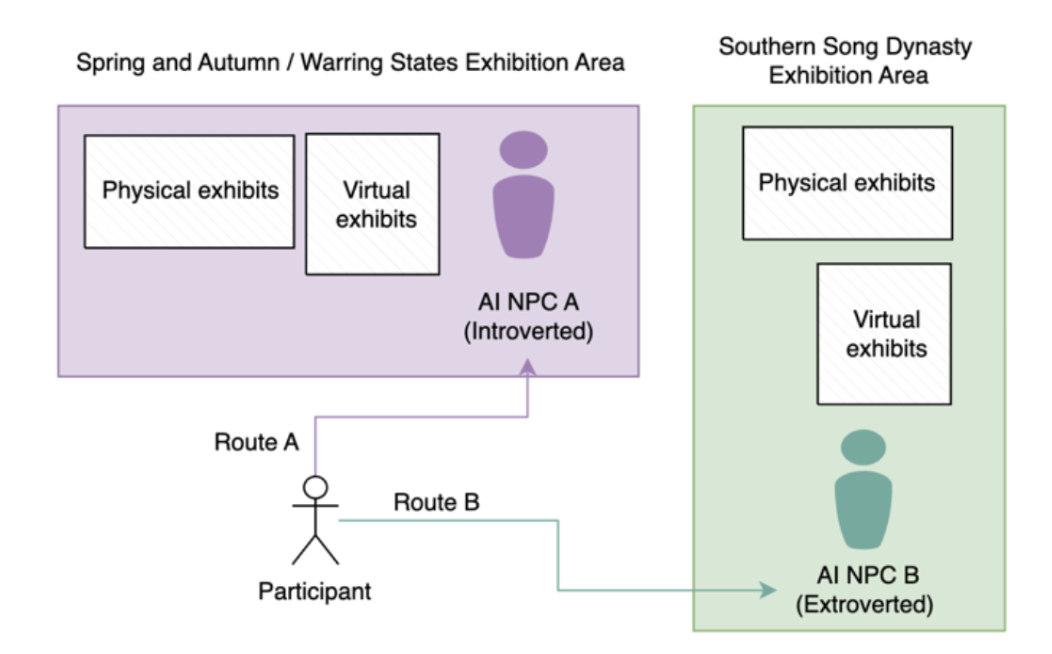
\includegraphics[width=0.5\linewidth]{figs/5.png}
    \caption{Caption}
    \label{fig:5}
\end{figure}

The physical layout of the study environment is presented in Figure \ref{fig:5}. To examine the impact of AI NPC personality traits on participant responses, this study employed both subjective (questionnaire) and objective (behavioral) measures. Objective data were collected through observation and MR device recordings, focusing on behavioral indicators linked to social presence (Biocca, 2003), which included (1) the number of AI– participant interactions, recorded by counting verbal and preset-prompt questions, and (2) eye-tracking metrics, which captured fixation counts and durations directed at three predefined Areas of Interest (AOIs): the AI NPC, physical exhibits, and virtual exhibits (Figure 6). Eye-tracking data enabled calculation of total gaze duration and engagement distribution across AOIs, providing a behavioral basis for assessing social presence.

\subsubsection{Result}

To investigate whether AI NPC personality influences perceived social presence (SP) in the MR tour, both objective data and subjective questionnaire responses were analyzed. Normality tests indicated that SP scores were approximately normal (p = 0.0942), but the small sample size (N = 16) limited parametric robustness. ITU, PI, and SAT scores were non-normal (p < 0.05). To ensure statistical validity, the Wilcoxon signed-rank test was used for all constructs. Given that over 10\% of scores were tied, two additional non-parametric methods—sign and permutation tests—were applied. All methods showed significant differences in SP between AI NPC personalities (p < .001), with extroverted AI receiving higher ratings (see Table 3 and Figure 7). These findings support H2a: Extroverted AI NPCs elicit higher levels of self-reported social presence compared to introverted AI NPCs.

\subsubsection{Discussioin}



\section{Pair}\label{sec:pair}

The formal study with single user examined how NPC personality shaped individual users’ perceptions and evaluations in an MR museum experience. However, museum visits are often social, and the presence of a partner may alter how users attend to and interact with the AI. Therefore, we conducted a dyadic pilot study to explore human–human–AI interaction and to inform the subsequent formal study.

\subsection{Pilot Study}
We conducted a pilot study at the Yang Ming Oceanic Culture \& Art Museum in Keelung, Taiwan, to explore how AI NPCs may shape collaborative interaction in a shared MR museum context. The study involved three acquainted pairs, resulting in a total of six participants. Using Microsoft HoloLens 2, each pair experienced a co-located MR museum environment in which they could interact with physical artifacts, virtual exhibit content, and two exhibit-specific AI NPC guides. 

The two NPCs were designed with contrasting personality styles based on the Big Five dimension of extraversion \cite{Neffetal2010}. The introverted NPC was embodied as Emperor Huizong of Song, while the extroverted NPC was embodied as Emperor Qianlong. Both NPCs were connected to exhibit-specific knowledge through retrieval-augmented generation (RAG) to support historically grounded responses.

The experimental design was guided by the following goals:
\begin{itemize}
    \item To position the AI NPCs as exhibit-specific historical guides rather than general-purpose chatbots.
    \item To encourage human-human collaboration through asymmetric clue distribution.
    \item To examine whether NPC personality, especially extraversion, could influence users’ social perception, AI reliance, and collaborative engagement.
\end{itemize}

To design the NPCs as supportive guides that provide hints and scaffolding rather than directly giving task answers.
Based on these goals, the experimental design centered on two main components: personality design and collaborative task design.

\subsubsection{Personality Design}

AI NPC personality was operationalized as the primary within-pair independent variable. Drawing on the Big Five personality framework, we focused on extraversion as the target dimension for personality design, following prior work on personality perception in conversational agents. The manipulation was implemented through both language and speech design. At the language level, GPT-4 prompts were used to specify each NPC’s conversational style, degree of proactivity, and emotional expressiveness. At the speech level, Azure TTS parameters were adjusted to further differentiate the perceived interaction style of the two NPCs.

In the introverted condition, the NPC was designed to provide more concise responses, adopt a reserved conversational style, and express lower emotional intensity. In the extroverted condition, the NPC was designed to use more enthusiastic language, initiate interaction more proactively, and display higher emotional expressiveness. Although each NPC was also embedded within an exhibit-specific historical identity, the core manipulation centered on contrasting introverted and extroverted interaction styles.

\subsubsection{Collaborative Design}

We designed a clue-based task related to the exhibits which intended to encourage collaboration within pairs in a shared MR museum context. Each participant received the same background story and task questions but was provided with different exhibit-related clues. This asymmetric information structure made collaboration necessary, as participants had to exchange information, discuss their interpretations, and coordinate their next steps in order to progress through the task.

To support this collaborative structure, we further constrained the NPCs’ task-related behavior through system prompts. The NPCs were instructed to recognize the ongoing collaborative task, avoid directly revealing the answer, and provide indirect hints instead. They were also prompted to treat the interaction as a multi-user conversation and to consider the shared conversation history when responding.

\subsubsection{Findings}

\begin{table}[htbp]
\caption{Participant demographics and extraversion characteristics}
\label{tbl:participant_demographics}
\begin{tabular*}{\tblwidth}{@{\extracolsep{\fill}}lccc@{}}
\toprule
 & \textbf{Overall}
 & \textbf{Introvert users}
 & \textbf{Extrovert users} \\
\midrule
\textit{N}
    & 6
    & 2
    & 4 \\

Male, \textit{n} (\%)
    & 5 (83\%)
    & 2 (100\%)
    & 3 (75\%) \\

Female, \textit{n} (\%)
    & 1 (17\%)
    & 0 (0\%)
    & 1 (25\%) \\

Age, \textit{M} (\textit{SD})
    & 23.5 (0.5)
    & 23.5 (0.7)
    & 23.5 (0.6) \\

Age, range
    & 23--24
    & 23--24
    & 23--24 \\

Extraversion, \textit{M} (\textit{SD})
    & 3.32 (0.66)
    & 2.55 (0.13)
    & 3.70 (0.37) \\

Extraversion, range
    & 2.45--4.00
    & 2.45--2.64
    & 3.18--4.00 \\
\bottomrule
\end{tabular*}
\end{table}

The demographic information is shown in Table \ref{tbl:participant_demographics}. The pilot study included six participants: five males and one female. Participants were between 23 and 24 years old, with a mean age of 23.5 years (SD = 0.5). Based on self-reported extraversion scores, two participants were categorized as introvert users and four as extrovert users. The introvert users had lower extraversion scores (M = 2.55, SD = 0.13) than the extrovert users (M = 3.70, SD = 0.37), providing a descriptive basis for exploring how users with different trait extraversion levels responded to the AI NPCs.

\subsubsection{Limitations}

The pilot study revealed several limitations in both the system implementation and study design. First, several participants experienced difficulty manipulating the MR interface. In particular, some participants were unable to reliably press the virtual speech-input button, which disrupted their ability to initiate conversations with the AI NPCs. This usability issue suggested that the input mechanism and system-status feedback needed to be made clearer and more robust.

Second, although the NPC personalities were explicitly encoded through prompts and validated using BFI-based assessments, participants did not always perceive the introverted and extroverted NPCs as intended. This suggests that prompt-based personality design alone may not be sufficient to produce consistent perceived personality in embodied MR interaction.

Third, the task-related prompting strategy was overly conservative. Because the NPCs were instructed not to reveal answers directly, some hints became too indirect, making the task difficult for participants to solve. This indicated the need to better balance answer withholding with useful scaffolding.

Finally, all participant pairs in the pilot study were acquainted with each other. As a result, the observed interaction dynamics may have been shaped by pre-existing social relationships, making it difficult to determine whether similar patterns would emerge among unfamiliar pairs.

\subsubsection{Design Refinements After the Pilot}

Based on these limitations, we refined both the system design and the study design before conducting the subsequent experiment. First, we expanded participant recruitment to include both acquainted and unacquainted pairs, allowing us to examine how prior familiarity may shape collaborative interaction with AI NPCs.

Second, we improved the speech-input interface by making system states more explicit. The interface was revised to help participants distinguish between available to speak, listening, processing, and responding states, thereby reducing uncertainty during turn-taking with the AI NPCs.

Third, we refined the personality prompts to strengthen the distinction between the introverted and extroverted NPCs. Specifically, the personality-related instructions were placed on the top in the prompt structure and marked as important to increase their priority during response generation. This refinement was intended to improve the consistency between the system-defined personality and participants’ perceived personality.
Finally, we adjusted the task-related prompting strategy to reduce task difficulty while preserving the collaborative structure. 

Instead of only providing indirect hints, the NPCs were allowed to offer more scaffolded guidance, such as presenting possible options or narrowing the range of interpretations. This refinement was intended to help participants progress through the task without allowing the NPCs to simply provide the correct answers.

\subsection{Experiment}

Building on the findings and design iterations from the pilot study, Study 3 conducted a formal evaluation of the dyadic MR experience with a larger sample of familiar and unfamiliar pairs. The study examined how NPC personality and pair familiarity shaped users’ perceptions of the AI, reliance on the NPCs, and collaborative engagement.


\subsection{Cross-Study Analysis}

To further comparing the collected data between single user and pair users, we seperate them into three group: single/acquainted pair/unacquainted pair. And we compared their Social Presence(SP), Intention to Use(ITU), and Satisfaction(SAT).

\begin{figure}
    \centering
    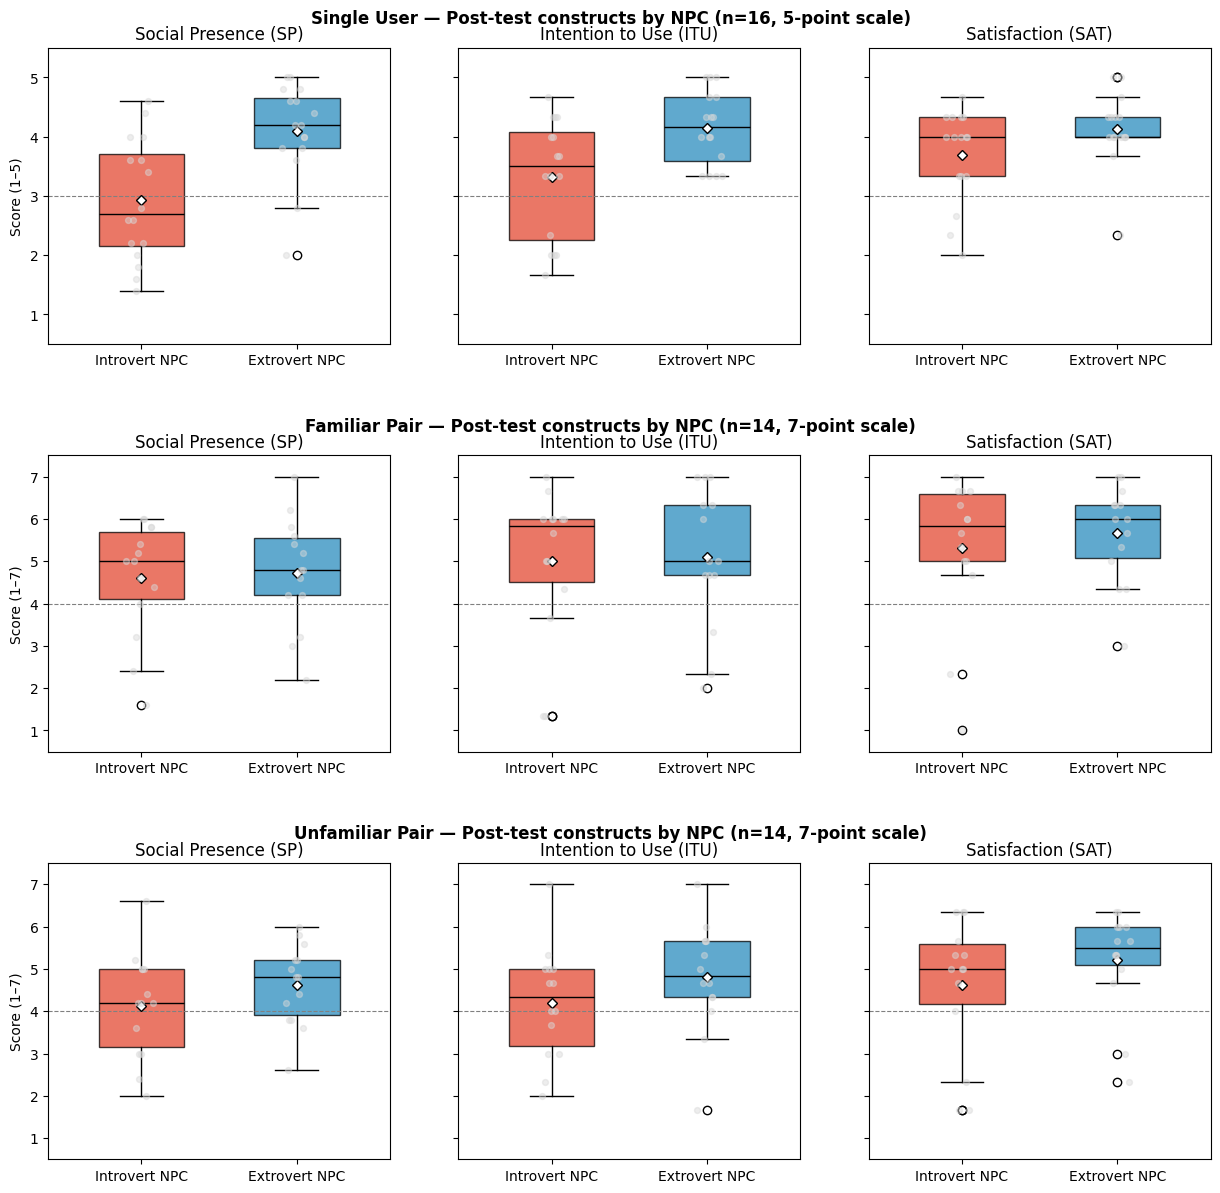
\includegraphics[width=0.5\linewidth]{figs/output.png}
    \caption{Boxplots of Average User Ratings for Introverted vs. Extroverted AI NPCs on SP, ITU, and SAT Constructs}
    \label{fig:boxplots}
\end{figure}

From figure \ref{fig:boxplots}, we can tell that overall, participants in the Single User condition exhibited a more pronounced advantage for the extroverted NPC in terms of social presence (SP) and intention to use (ITU). In contrast, the differences observed in the Familiar Pair and Unfamiliar Pair conditions were smaller and less consistent. This pattern suggests that when users interact with an NPC alongside another participant rather than individually, the influence of NPC personality on subjective evaluations may be attenuated by the presence of a human partner.

Because the Single User study employed a 5-point Likert scale, whereas the pair-based studies employed a 7-point Likert scale, all questionnaire responses were normalized to a common 0–1 scale for the subsequent analyses.

To further examine whether the effects differed statistically across the three interaction conditions, a difference score was calculated for each participant and construct by subtracting the rating of the introverted NPC from that of the extroverted NPC. A positive score therefore indicated a relative preference for the extroverted NPC, whereas a negative score indicated a relative preference for the introverted NPC.

Kruskal–Wallis tests were then conducted to compare the distributions of the difference scores across the Single User, Familiar Pair, and Unfamiliar Pair conditions. The results revealed a significant between-condition difference in the SP difference scores, indicating that the relative effect of the extroverted NPC, compared with the introverted NPC, on perceived social presence varied across interaction conditions.

By contrast, the Kruskal–Wallis tests for ITU and satisfaction (SAT) were not statistically significant. Thus, there was insufficient evidence to conclude that the relative advantage of the extroverted NPC in terms of intention to use or satisfaction differed across the three interaction conditions.


\subsubsection{Behavioral Result}

\subsubsection{Similarity Attraction Effect}

\section{General discussions}\label{sec:general}

\section{Conclusion, Limitations, and Future Work}

% % To print the credit authorship contribution details
% \printcredits

%% Loading bibliography style file
%\bibliographystyle{model1-num-names}
\bibliographystyle{cas-model2-names}

% Loading bibliography database
\bibliography{cas-refs}

% Biography
%\bio{}
% Here goes the biography details.
%\endbio

%\bio{pic1}
% Here goes the biography details.
%\endbio

\end{document}

